\RequirePackage{silence}
\WarningFilter{latex}{You have requested document class}
\WarningFilter{latex}{You have requested package}

\documentclass[UKenglish, twoside]{ifimaster}  %% ... or USenglish or norsk or nynorsk
\raggedbottom
\usepackage{fancyhdr}
\usepackage[utf8]{inputenc}           %% ... or latin1 or applemac
\usepackage[T1]{fontenc,url}
\usepackage{float}
\usepackage{hyperref}
\urlstyle{sf}
\usepackage{textcomp,csquotes,duoforside/duomasterforside,varioref,graphicx}
\usepackage[acronym, toc]{glossaries}
\usepackage{enumitem}

\renewcommand{\baselinestretch}{1.5}

%\usepackage[backend=biber,style=apa, citestyle=authoryear]{biblatex}
\usepackage[british]{babel}
%\usepackage{natbib}
%\usepackage{authordate}
\usepackage[backend=biber, style=apa, citestyle=authoryear, uniquename=false]{biblatex}
\DeclareLanguageMapping{british}{british-apa}

%\DeclareLanguageMapping{british}{british-apa}
\title{Empathy tools as a way to universal designed ICT solutions?}
%\subtitle{A critical exploratory study}
%\subtitle{Can empathy tools}
\author{Markus J. Sørem}
\makenoidxglossaries
%\makeglossaries
\newglossaryentry{UniversalDesign}
{
    name = Universal Design,
    description = {The design of products and environments to be usable by all people, to the greatest extent possible, without the need for adaptation or specialised design \parencite{miljoverndepartementet_t-1468_2007}}
}
\newglossaryentry{accessibility}
{
    name = accessibility,
    description = {That a service can be used by people with disabilities}
}
\newglossaryentry{disability}
{
    name = disability,
    description = { Disabilities, or impairments, are loss, damage on, or deviation of a body part, or in one of the body's psychological, physiological or biological functions (translated from \cite{barne-_ungdoms-_og_familiedirektoratet_hva_2015}}
}
\newglossaryentry{WCAG}
{
    name = WCAG 2.0,
    description = {Guidelines that specify how to make content accessible, primarily for people with disabilities}
}
\newglossaryentry{Human-Computer Interaction}
{
    name = Human-Computer Interaction,
    description = {Human-Computer Interaction (HCI) is a research field focused on the interfaces that enables interaction between humans and computer. Interfaces can be physical, digital or voice-based [FIND REFERENCE].}
}
\newacronym{hci}{HCI}{\Gls{Human-Computer Interaction}}
\newacronym{ffo}{FFO}{\Gls{Funksjonshemmedes Fellesorganisasjon}}

\newglossaryentry{Funksjonshemmedes Fellesorganisasjon}
{
    name = Funksjonshemmedes Fellesorganisasjon,
    description = {A Norwegian umbrella organisation for associations by people with disabilities and chronic illnesses.}
}
%\newacronym{difi}{Difi}{\Gls{Direktoratet for forvaltning og IKT}}
\newglossaryentry{difi}
{
    name =  difi,
    description = {Norwegian agency with a goal of modernising and adjusting the public sector. }
}


%%\addbibresource{bibliography/bibliography.bib}
%%\bibliographystyle{apalike}
%\bibliography{citations}                  %% ... or whatever
\addbibresource{citations.bib}
%\addbibresource{mendeley.bib}

\begin{document}
  
\duoforside[dept={Department of Informatics},   %% ... or your department
  program={Informatics: Design, Use and Interaction},  %% ... or your programme
  long]                                        %% ... or long

\frontmatter{}
%\chapter*{Abstract}                   %% ... or Sammendrag or Samandrag

\tableofcontents{}
\printnoidxglossary
%\listoffigures{}
%\listoftables{}

%\chapter*{Preface}                    %% ... or Forord

\mainmatter{}
\pagestyle{fancy}
\renewcommand{\chaptermark}[1]{%
\markboth{#1}{}}
\fancyhf{}
\fancyhead[RO]{\emph{\nouppercase{\leftmark}}}
\fancyhead[LE]{\emph{\hyperlink{toc}{Chapter \thechapter}}}
\setlength{\headheight}{14.50pt}% ...at least 51.60004pt
\cfoot{\thepage}

%\part{Introduction}
%\chapter{Introduction}

\chapter{Introduction}
\epigraphhead[20]{\epigraph{\textit{"It means very little to know that a million Chinese are starving unless you know one Chinese who is starving."}}{{\textbf{John Steinbeck}}}}

%\chapter{Background}

\section{The story of Sven}
Sven is from Sweden, but has recently moved to Norway because of work. During his stay he has come across Norwegians from different parts of Norway, all using words that are unfamiliar to him. Most Norwegians can't expect Sven to understand these words, so they intuitively adapt their communication when speaking to him. Sven, on his side, cannot expect Norwegians he meets to speak Swedish to him and he also has to adapt by using words Norwegians understand. This mutual understanding comes from Sven interacting with Norwegians and from Norwegians empathy with Sven as a foreigner. If this was a one-way conversation, Norwegians wouldn't know that Sven had troubles understanding them, and Sven would have a harder time living in Norway.

\section{Background}
%Digital public services has the potential to increase productivity by automating communication between citizens and public services, and between businesses and public services, according to \textcite{Moderniseringsdepartementet2016}.

Information and communication technology (ICT) is integrated in nearly all parts of modern society. 
92\% of Norwegian citizens had access to the Internet in 2011 and 79\% used it daily. In 2015 97\% had access to the Internet and 90\% used it daily. In three years, time spent on the Internet has grown from 112 minutes (in 2013) to 140 minutes (in 2016) per person on average \parencite{ssb_tid_2017}. The use of digital public services has increased by 235\% from 2010 to 2015 \parencite{Moderniseringsdepartementet2016}. 

But there are large differences in age. 44\% of the group between 75 - 79 years report not using the Internet and only 4\% say they have good skills in using the Internet. "Digital natives" (young people grown up using digital devices) can also struggle when an unclear language is used in the digital sphere \parencite[40]{Moderniseringsdepartementet2016}.

Most people are online all the time and expect instant access to information and services. It is important that ICT services are designed and built in a way that does not exclude people with different prerequisitions. Autonomy, equality and inclusion are all important aspects to keep in mind when we are moving towards a more digital society.

Universal design is an attitude and a tool with the intent to include most people in society regardless of functional abilities, age or education. The intent is not to make separate or "special solutions", but to make the same solution accessible and usable by the largest amount of users. 

There has been an increased awareness and interest in Universal Design of ICT in Norway the last couple of years \parencite{begnum_universal_2017}. Awards such as Doga’s (Design and Architecture Norway) “Innovation price for Universal Design” are dealt to ICT solutions who has “made Norway a more including and open society” (Grafill, 2017). Norway has legislated that all new solutions aimed at the general public must be universal designed and all existing solutions must be universal designed by 2021 \parencite{ministry_of_children_and_equality_act_2018}. However, in a report checking the status of universal design of both private and public ICT solutions in Norway, 54\% of public and 49\% of private solutions were measured as being universal designed with scores ranging from 18 to 79 percent \parencite{difi_digitale_2015}.

%\textcite{Cardoso2012} 
%The reason

%Using a user-centered design approach is often the recommended way to meet universal design guidelines (\cite{fuglerud_link_2013 , Keates2014}). But in practise, inclusion of users with different impairments can be hard to accomplish due to availability and budget/time constraints. As a consequense 

%How disability and impairments are viewed by the people making ICT solutions can affect the quality and degree of universal design. Can empathy tools simulating impairments teach empathy? Can the first hand experience of difficulties by using an ICT solution change views developers might have on people with disabilities? 


%Can sympathy, empathy and compassion be used to explicitly state how 

%Can challanging views developers have on universal design and disabilies be a 

%How disability and impairments are viewed by the people making ICT solutions can affect the quality and degree of universal design






%From bank services to building permits, everything is mostly done digital. Norway is the most digitised country in the world \parencite{dagens_naeringsliv_norge_2017}, and it is important to ensure inclusion of all members of society, including people with various forms of disabilities.  


%The fear of breaking the law and to have to remake ICT solutions has also incentivised ICT professionals to focus on Universal Design. However, only 51\% of 300 websites evaluated by Difi in 2015 was within the requirements of the government in Norway.

%\Gls{accessibility} on the web has come a long way in a few decades. It is now punishable by law in Norway to make a publicly accessible website without meeting the criterion for \Gls{UniversalDesign}, and all existing websites must follow these criterion by 2021. But it can be hard to measure if a website is universal designed or not, and to make sure they stay this way when they get updated over time.

%Norway has come a long way legally when it comes to inclusion in the digital sphere. Norway legislated the Anti Discrimination and Accessibility Act in 2008 demanding ICT solutions aimed at the general public to be accessible. Difi (no: Direktoratet for forvaltning og IKT, en: Agency for Public Management and eGovernment) has the role of evaluating existing solutions using the WCAG (Web Content Accessibility Guidelines) 2.0 technical standard.

%\section{Universal Design}
%Many terms for designing and developing ICT solutions that can be used by as many people as possible exists, like "Universal Design", "Universal Usability", "Universal Access", "Design for All" and "Inclusive Design" \parencite{fuglerud_link_2013}. This thesis uses \textbf{universal design} as an umbrella term for all these approaches because The Norwegian Directorate for Children, Youth and Family Affairs (Bufdir) says that these terms are synonymous \parencite{bufdir_universell_2017}. Universal design is also the term used in 

\section{Motivation}
Adherence to requirements and standards is a frequently used approach to universal design \parencite{fuglerud_link_2013}. While this is often a precondition, it does not solve the whole problem. For example: conformance to WCAG 2.0 guidelines can only solve around half of the issues experienced by visually impaired users. Fuglerud suggests that the requirements are used as a part of a human-centered design (UCD) process. This process incorporated in ISO (the International Organization for Standardization) 9241-210:2010 focuses on the use of the system and include the user in the design and development process.

But inclusion of users with different impairments can be hard to accomplish due to availability and budget/time constraints.





%The motivation to conduct this research comes from both a professional and personal level. The professional reason to learn about Universal Design, is that I want to be ready to work as as an interaction designer after I graduate. During the study, I have found out that Universal Design isn’t always focused on early on in projects unless the team has someone who has an understanding and motivation to make sure the team focuses on Universal Design principles.

%PERSONAL MOTIVATION
%My personal motivation to conduct this research comes from an empathy for a group of people who are not always heard. My mother has worked with cultural activity for people with mental and physical disabilities, and has let me participate in her work since I was a child. Aside my studies, I have worked as a social worker with people with autism. With my background I would say that I have empathy for people with different kinds of impairments, and would like to make the world a little better place to live in for this group. 


%\begin{displayquote}
%Disability is not the impairment itself, but rather attitudes and environmental barriers that result in disability.

%- Unicef
%\end{displayquote}

%The Norwegian Equality and Anti-Discrimination Act aims to \textit{"help to dismantle disabling barriers created by society and prevent new ones from being created."} This includes dismantling digital barriers. The legislation views disability as happening when society does not meet the requirements of the individual. This is known as the social model. 

%Contradicting this view is the medical model seeing disability as something within an individual needing treatment in order to be "fixed" \parencite{begnum_2016_views}.




%In Norway, the criteria for an ICT solution to be regarded as universal designed is that it has to follow the WCAG 2.0 technical standard. \textcite{fuglerud_link_2013} states that although guidelines such as WCAG 2.0 is a precondition to achieve an accessible solution, it might not always be enough. A solution might be technically or theoretically within the requirements of universal design, but still be difficult to use. Some research suggests that WCAG 2.0 only covers around half of the issues encountered by visually impaired users \parencite{fuglerud_link_2013}. 

%\subsection{Views on disability}
%The Norwegian Equality and Anti-Discrimination Act aims to "help to dismantle disabling barriers created by society and prevent new ones from being created." This includes dismantling digital barriers. \textcite[]{begnum_2016_views} says that this legislation is based on a modern right view on disabilities which thinks that everyone should have equal rights and not be discriminated against. The legislation is also based on a social adapted model promoting the dismantling of social constructed barriers.

%\textcite{begnum_2016_views} was surprised when she found out that 77\% of the participants (universal design experts) in her study agrees %(amongst other) with the \textbf{charity model} viewing disability as unworthy, a personal tragedy, and that "disabled persons deserve sympathy, support and help". She also notes that this view is common amongst non-disabled people.

%The social adapted model sees contextual and environmental factors as creating the largest barriers for inclusion, while the charity and the closely related medical model focus more on the individuals impairments. The medical and the charity model are according to Langtree (2010 in \cite{begnum_2016_views}) the most common model used by non-disabled people to define and explain disability. 

\subsection{Empowering developers}
The focus of this thesis is frontend developers working on ICT solutions. The reason for this is that it is often up to frontend developers if the ICT solutions are universal designed or not, especially when it comes to semantic code 

Frontend developers of web based ICT solutions in the private sector is the focus of this project. The private sector 

The reason for this is that it is often up to frontend developers if the ICT solutions are universal designed or not, especially when it comes to semantic code. In the evaluation of \textcite{difi_digitale_2015}, code related accessibility errors was found to be most common. Wrong use of heading tags, 

%The legislated requirements used to evaluate ICT solutions can be appear fuzzy \parencite{begnum_universal_2017}, developers typically have little to no training in making ICT solutions user friendly \parencite{Law:ProgrammerFocusedWebsiteAccessibilityEvaluations:2005} and courses aimed at engineers and ICT students in usability and universal design are only available at some universities and are almost always electives \parencite{Jordan2010}.

\textcite{Freire2008} says accessibility has been a very important issue in web development, but that there is a lack of knowledge among developers on which techniques should be used to make websites accessible. They suggests teaching developers how individuals use assistive technologies and show them how a target user struggles with their solutions.

\subsection{Personal motivation}
My personal motivation to conduct this research comes from an empathy for a group of people who are not always heard. My mother has worked with cultural activity for people with mental and physical disabilities, and has let me participate in her work since I was a child. Aside my studies, I have worked as a social worker with people with autism. With my background I would say that I have empathy for people with different kinds of impairments, and would like to make the world a little better place to live in for this group. 

%Langtree (referred to in \textcite{begnum_2016_views}) states that charity 

%\subsection{Why focus on developers}
%As \parencite[]{lundstrom_perceptions_2015} notes, developers tend to take their own decisions when it comes to design

%\section{Goal}
%The ultimate goal for conducting this research is making universal design principles relevant for developers, make it easier to learn about universal design principles and to ultimately on their own be able to identify accessibility issues that automatic testing tools fails to identify. One way to meet this goal is to find a way to lower the threshold for front-end developers to make universal designed ICT solutions. By introducing empathy tools that simulates different types of impairments developers can experience first-hand how an ICT solution might be experienced, to some degree, by people who has disabilities. Can these tools, when used on a prototype or solution the developer has made, have an impact into their views on disability and digital inclusion?

\section{Research Questions}
%The ultimate goal for conducting this research is to understand how empathy tools might impact developers. 

The ultimate goal for this project is to understand how to motivate more developers to assimilate a universal design mindset. My hypothesis is that by letting developers use tools that can simulate functional impairments while using ICT solutions, this can make them realise where the solution is creating digital barriers and how this can be avoided. This knowledge can then be used in future projects.

%is making universal design principles relevant for developers and make it easier to learn about universal design principles so that developers on their own are able to identify accessibility issues that automatic testing tools fails to identify. My hypothesis is that by letting developers use tools that can simulate functional impairments while using ICT solutions, this can make them realise what the digital barriers in the solutions are and how they might be perceived by people who have different kinds of impairments. This again can make it easier to recognise such barriers in other ICT solutions

%The ultimate goal for conducting this research is making universal design principles relevant for developers and make it easier to learn about universal design principles so that developers on their own are able to identify accessibility issues that automatic testing tools fails to identify. My hypothesis is that by letting developers use tools that can simulate functional impairments while using ICT solutions, this can make them realise what the digital barriers in the solutions are and how they might be perceived by people who have different kinds of impairments. This again can make it easier to recognise such barriers in other ICT solutions

%One way to meet this goal is to find a way to lower the threshold for front-end developers to make universal designed ICT solutions. By introducing empathy tools that simulates different types of impairments developers can experience first-hand how an ICT solution might be experienced, to some degree, by people who has disabilities. Can these tools, when used on a prototype or solution the developer has made, have an impact into their views on disability and digital inclusion?

%To lower the threshold of making universal designed ICT solutions, I first have to understand how universal design is dealt with in the development process, and how it should be dealt with. 

%My first research question is:

%\textit{What are the main constraints or barriers hindering developers from making more accessible ICT solutions?}
%\textit{Can empathy tools be a way of empathising}
%\textit{What are the main factors involved in projects that successfully integrates universal design and accessibility?}

\begin{enumerate} 
\item \textit{How to make accessibility issues more apparent for ICT students or professional developers?}
As 
%\item \textit{What are the main factors hindering or promoting developers in making universal designed ICT solutions?}
\item \textit{Can empathy tools motivate the developers to consider the needs of people with different capabilities?}
    \begin{enumerate}
        \item What needs to be present to enable developers to be motivated?
    \end{enumerate}
\end{enumerate} 

 
%My first research question:  


\begin{enumerate} 
%\item \textit{What are the main factors hindering or promoting developers in making universal designed ICT solutions?}
\item \textit{How does the use of empathy tools impact developers?}

\end{enumerate} 
By letting frontend developers use empathy tools on different ICT solutions, I aim at getting a better understanding on the impact this experience have.
%I'm also exploring the use of empathy tools which simulates various impairments and hope to see if this can impact the views front-end developers might have on people with disabilities. 
%I also want to review existing software simulators with developers to see if they can be helpful in their work on developing Universal Designed ICT solutions.

%The technical standards used to evaluate ICT solutions can be hard to fathom, and the most common way used by developers to make sure an ICT-solution is accessible and meeting guidelines and best practises in ICT-projects, is using automatic testing tools that gives feedback on the quality on \textit{code itself} with regards to being technical accessible by for example screen readers.

%Automatic testing tools are valuable in some degrees, for example in making sure all images on a website has an existing alternative text. However, human cognition and usability can not be tested automatically - we then need to think about how the end-user can experience the solution. 

%Empathy is described as understanding the other and seeing a situation from the perspective of others \parencite{lundstrom_perceptions_2015}. My hypothesis is that simulations can provide some low-cost insight into the experience others might have with the artefact. By introducing developers to simulation techniques they can use in their work on ICT-solutions, it can expand their understanding of the diverse abilities and disabilities of people who can become end-users of their solutions and to see the solution from their perspective. Simulations can also make it easier to recognise accessibility issues earlier and learn how to recognise these issues in later projects.

There are many kinds of empathy tools aimed at conveying how different impairment might be experienced. In terms of usability and cost/benefit factors, I analyse which tools might suit frontend developers best.

My second research question is therefore:
\begin{enumerate}\addtocounter{enumi}{1}
\item \textit{Which kinds of empathy tools are best suited for developers working on ICT solutions?}
\end{enumerate} 
%Through a deep dive into existing research on the topic, I hope to explain how simulations can be used in the context of working with ICT-solutions with a frontend developer-centered focus.

%There are many existing simulation techniques and simulation software, and I want to evaluate these with frontend developers. The end goal would be to have requirements of a simulator that is fitting the needs of the developer, and that can help making sure the solution adheres to laws, guidelines and best practises. My third research question is therefore:
%\begin{enumerate}\addtocounter{enumi}{2}
%\item Which simulation techniques or software can be used to make it easy and cost-beneficial for frontend-developers working with ICT-solutions.
%\end{enumerate}
%Simulating impairments means that prototypes can be evaluated by humans, rather than automated testing tools. Many accessibility issues can be found before real users are introduced to the prototype, and the designers and developers can be trained to build ICT solutions more accessible.
%The thesis also has a practical part where I want to build a simulator and evaluate this by including developers and designers and following a User Centered Design (UCD) process.
% where it should be used
% who will be using it
% what are the requirements
% simulating the use of the simulator??
\chapter{Theory}
This thesis is placed in the field of \acrfull{hci}. Themes and methods used in this thesis, are therefore mostly connected to HCI.

The thesis is written with a Norwegian perspective in mind, and most theory, examples and data will therefore be in the context of Norway and the Norwegian population. 

\section{Interaction Design and \acrfull{hci}} 
\acrshort{hci} is an academic field concerned with "understanding the influence technology has on how people \textit{think, value, feel and relate}" and how this understanding can inform the design of technology \parencite{wright_empathy_2008}. Interaction Design is the industrial adaptation of HCI research, and is concerned with the practical design of products with the ultimate goal of supporting people (end users) in their everyday and working lives \parencite{rogers_interaction_2011}.

Both HCI and Interaction Design is concerned with understanding people and how they use ICT solutions and how the user experience can be improved in existing solutions or intact/integrated in future solutions.

%user experience

%empathy
%sympathy


\section{Regulations and guidelines}
In Norway, a regulation concerning Universal Design was passed in 2013 (Kommunal- og moderniseringsdepartementet, 2013). According to \Gls{difi} the vision of having this regulation is to have a society without digital barriers \parencite{difi_digitale_2015}. Digital barriers refers to the hinderings some people with impairments experience using technology, and it comes according to \textcite{malin_rygg_dei_2015} mostly from bad coding, low contrast and lack of textual alternatives for illustrations on websites. 

\subsection{Discrimination and Availability Act}
The Norwegian legislation "Discrimination and Availability Act" (no: Diskriminerings- og tilgjengelighetsloven) came in effect 1. January 2009. The legislation states that "equality, equal opportunities and community engagement should be available to all, independent on functional abilities". The law also makes sure to hinder discrimination because of disabilities.

According to the legislation, ICT-solutions that are aimed at the public must be universal designed by 1. Juli 2011. Existing solutions must be universal designed by 1. January 2021 \parencite{_lov_2013}. Failure to meet this deadline might result in a coercive fine \parencite{_lov_2013}.

\subsection{WCAG 2.0 guidelines}
The extent to if, and how well universal designed a website or application is, is in Norway measured by using the \Gls{WCAG} (Web Content Accessibility Guidelines) 2.0 technical standard. Norwegian websites (and some applications) that are aimed at Norwegian citizens, are used to inform or offer services, and is new or published after 1. July 2014, are all affected by this regulation. Providers of websites and applications that are older than this have until 1. January 2021 to meet the WCAG 2.0 requirements (ibid).
\Gls{WCAG} is based on four top principles:
\begin{itemize}
    \item Perceivability
    \item Operability
    \item Understandability
    \item Robustness
\end{itemize}

Under these principles are guidelines that explain the goals each success criteria should meet. WCAG 2.0 includes testable success criterion in three levels: A, AA and AAA, which are separated in the degree the success criterion impacts the design of the website. Most AA success criterion are included in the regulation on universal design of ICT solutions. %cite the regulation


\section{Definitions and wording}
\subsection{Sympathy vs. empathy}
Empathy can be described as "understanding the other and seeing a situation from the perspective of others" \parencite{lundstrom_perceptions_2015}.  

%skriv om hvordan man får til empati etc.

%\textcite{wright_empathy_2008} notes that the first view of empathy, identify and becoming the user, 


\subsection{Accessibility and Universal Design}
Accessibility and Universal Design are related terms. Accessibility is concerned with whether a solution has the properties of being usable by people with impairments. \textcite{paddison_applying_2003} separates technical and usable accessibility. Technical accessibility is making sure the solution are usable by assistive technology, such as screen readers, by adding alternative text, using scalable measures in font sizes et cetera. Usable accessibility is ensuring a good user flow, consistent layout and more.

When ICT-solutions are accessible \textit{and} usable (that it governs both technical and usable accessibility) to a larger part of the population, it is often referred to as being “Universally Designed”. The Norwegian Environmental Protection Agency defined Universal Design in 2007 as “...the design of products and environments to be usable by all people, to the greatest extent possible, without the need for adaptation or specialised design” \parencite{miljoverndepartementet_t-1468_2007}. This means that the same solution should be usable for people with different functional levels. 

As an example: if a website with 500 links is accessible with the use of a screen reader, it can be said to be accessible. If the same website is usable for the people using the screen reader, without them having to go through all the 500 links to execute a task, it can be said to be Universal Designed. 

This is an oversimplification of the terms, and it all depends on the user, their abilities, the technology, the setting the technology is used and many other factors. Universal Design of ICT has the ultimate goal of making ICT accessible and usable for a given target group in an appropriate way \parencite{tollefsen_web_2013}, and to lower the digital barriers of the society. 

%\textcite{tollefsen_web_2013} defines Universal Design of ICT as “...development of products and services so that all people in a given target group can use the technology in an appropriate way”.

%In Norway, a regulation concerning Universal Design was passed in 2013 (Kommunal- og moderniseringsdepartementet, 2013). According to \Gls{difi} the vision of having this regulation is to have a society without digital barriers \parencite{difi_digitale_2015}.

%\Gls{UniversalDesign} as a concept began, according to \textcite{tollefsen_web_2013} at The Center for Universal Design at the end of 1980s. In Norway it began with the publication "Universal Design - planning and design for all" from 1997. %\gls{disability}.


\subsection{Disability and impairments}
Most people, especially in Norway, can expect access to education, employment, public transport and information. This is not necessarily the case for people who live with disabilities. According to \textcite{world_health_organization_world_2011} around 15\% of the world's population live with some sort of disability. This number is also growing because people are generally getting older, and older people have a higher risk of being disabled. 

\acrfull{ffo} defines disability as a conflict between an individuals premise to function and the environments requirements to function \parencite{funksjonshemmedes_fellesorganisasjon_ffo_definisjon_2013}. The Gap Model \ref{fig:gap_model} illustrates this conflict: 
\begin{figure}[H]
\minipage{1\textwidth}
  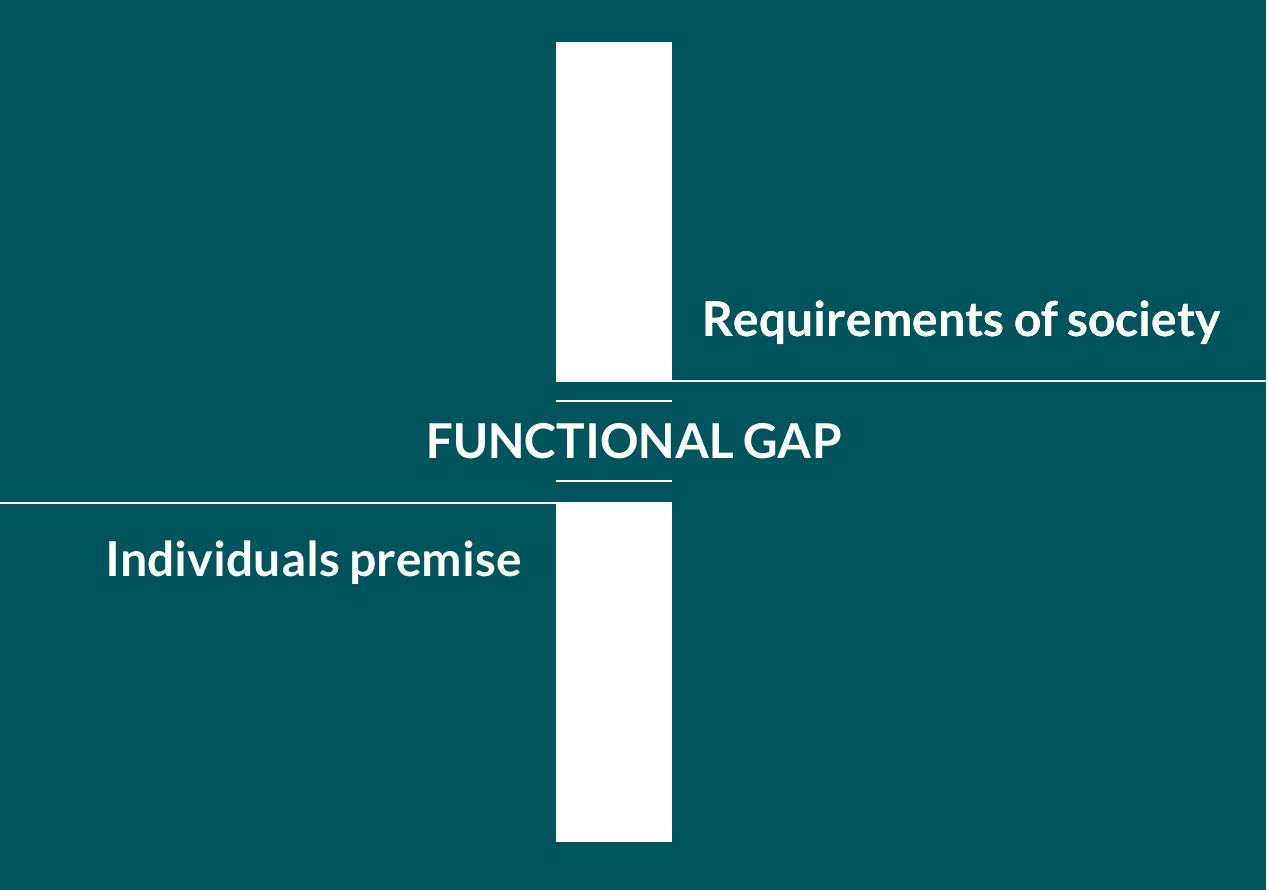
\includegraphics[width=\linewidth]{img/gapmodel.png}
  \caption{The Gap Model. Graphic based on \textcite{difi_kvifor_2016}.}\label{fig:gap_model}
\endminipage\hfill
\end{figure}
In order to decrease the functional gap, requirements of the society must be lowered. A way of doing this is to make sure ICT solutions are universally designed so that most people are able to participate in society. 
It is important to distinguish the terms "disability" and "impairment" as these are often used interchangeably \parencite{sheena_l._carter_impairment_????}. \textbf{Impairment} refers to "any loss or abnormality of psychological, physiological or anatomical structure or function." while \textbf{disability} refers to "any restriction or lack (resulting from an impairment) of ability to perform an activity in the manner or within the range considered normal for a human being" (ibid). 

More clearly, \textbf{impairment} refers to the \textit{physical} or \textit{cognitive} hindering/restriction of functionality the individual may have, while \textbf{disability} refers to the restriction the individual have to perform certain \textit{activities} or \textit{tasks}, because of the impairment. With this definition in mind, one can say that inaccessible environments \textbf{disables people} with impairments, not that the person are disabled because of their impairment. \textcite{world_health_organization_world_2011} also discusses this idea using the models "medical" and "social" where medical are the impairments the person may have, while the social model refers to the hinderings caused by society (the functional gap).

\subsection{Universal Design, Inclusive Design and all the above}

\iffalse
    \section{Disabilities and impairments}
    Most people, especially in Norway, can expect access to education, employment, public transport and information. This is not necessarily the case for people who live with disabilities. According to \textcite{world_health_organization_world_2011} around 15\% of the world's population live with some sort of disability. This number is also growing because people are generally getting older, and older people have a higher risk of being disabled. 
    
    \acrfull{ffo} defines disability as a conflict between an individuals premise to function and the environments requirements to function \parencite{funksjonshemmedes_fellesorganisasjon_ffo_definisjon_2013}. The Gap Model \ref{fig:gap_model} illustrates this conflict: 
    \begin{figure}[H]
    \minipage{1\textwidth}
      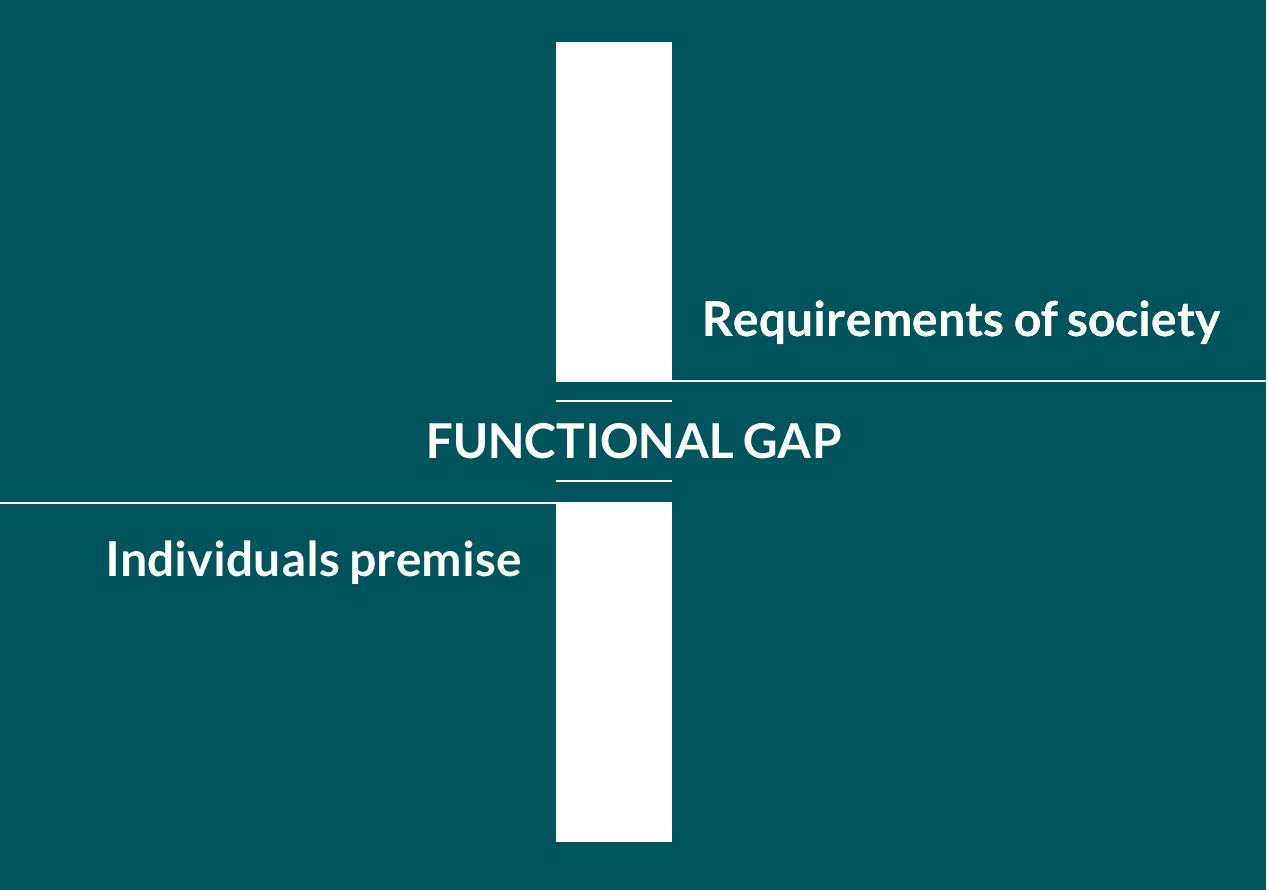
\includegraphics[width=\linewidth]{img/gapmodel.png}
      \caption{The Gap Model. Graphic based on \textcite{difi_kvifor_2016}.}\label{fig:gap_model}
    \endminipage\hfill
    \end{figure}
    
    In order to decrease the functional gap, requirements of the society must be lowered. A way of doing this is to make sure ICT solutions are universally designed so that most people are able to participate in society. 

\fi

\subsection{Impairments and disabilities}
It is important to distinguish the terms "disability" and "impairment" as these are often used interchangeably \parencite{sheena_l._carter_impairment_????}. \textbf{Impairment} refers to "any loss or abnormality of psychological, physiological or anatomical structure or function." while \textbf{disability} refers to "any restriction or lack (resulting from an impairment) of ability to perform an activity in the manner or within the range considered normal for a human being" (ibid). 

More clearly, \textbf{impairment} refers to the \textit{physical} or \textit{cognitive} hindering/restriction of functionality the individual may have, while \textbf{disability} refers to the restriction the individual have to perform certain \textit{activities} or \textit{tasks}, because of the impairment. With this definition in mind, one can say that inaccessible environments \textbf{disables people} with impairments, not that the person are disabled because of their impairment. \textcite{world_health_organization_world_2011} also discusses this idea using the models "medical" and "social" where medical are the impairments the person may have, while the social model refers to the hinderings caused by society (the functional gap).


\textcite{begnum_universal_2017} also mentions this difference between the medical and social model, where the medical model are concerned with what is wrong with a person, while the social model is concerned with what is wrong with society the individual is a part of. She says "it is a \textbf{social responsibility} to ensure that different physical and psychological abilities are taken into consideration and barriers are removed and diminished". 



%få med modell fra Jo - Gdrive

\subsection{Types of disabilities}
\Gls{difi} categorises four main groups of disabilities and how they can hinder people from using technology:
\begin{itemize}
    \item Motoric 
    
    Disabilities regarding movement and motorics. People in this category are sometimes in need of other types of interaction methods other than mouse, touch screen, keyboard or buttons in order to operate digital devices; for example eye tracking, joysticks or other alternative interaction methods.
    \item Visual
    
    People who experience visual impairments are people who, to some degree, have problems seeing or who are totally blind. This group consists of people with, amongst others, colour blindness, blurred vision or poor eyesight. 
    
    People with visual impairments can have problems with small text, small touch/click areas, unusual fonts etc. This group can also struggle when colours are the only differentiating factor between elements, or when contrast between elements are too low. 
    \item Auditory
    
    Auditory impairment refers to having problems hearing or being deaf. People with auditory impairments can have problems hearing the audio track of videos, sound clips or music, and needs the information presented textual or with sign language. 
    
    \item Cognitive
    
    This category involves people with problems processing information. Cognitive impairments involves: memory problems, concentration problems, learning problems, literacy problems etc. This group can be in need of other information
\end{itemize}

However, as noted by \textcite[p. 22]{world_health_organization_world_2011} people with the same type of impairment may have different experiences and needs. \\ 

%\textbf{SKRIV MER OM DETTE}

\noindent
In the Norwegian population:
\begin{itemize}
    \item 15\% in 2017 says they have impairments \parencite{barne-_ungdoms-_og_familiedirektoratet_antall_2017}
    \item [\textbf{Vision}]
        \item 180.000 live with a vision impairment \parencite{blindeforbundet_fakta_????}
        \item Over 1000 are color blind \parencite{blindeforbundet_fakta_????}
        \item 70\% of people over 70 develops cataracts \parencite{blindeforbundet_fakta_????}
    \item [\textbf{Cognitive}]
        \item 2.5\% adults has ADHD \parencite{adhd_norge_voksen_????}
        \item Around 5\% has dyslexia, 5\% has dyscalculi and 5\% has SSV \parencite{dysleksi_norge_fagstoff_????}
    \item [\textbf{Language}]
        \item 725.000 are first generation immigrants which most likely has another mother tongue than Norwegian \parencite{statistisk_sentralbyra_nokkeltall_2017}
    \item [\textbf{Age}]
        \item 220.000 people in 2017 are 80 years or older, 505.000 people are between 75 and 79 years old \parencite{folkehelseinstituttet_andelen_2017}
\end{itemize}
These statistics show that there is a large amount of the Norwegian population who lives with different kinds of impairments. \\

\noindent
Everyone will most likely experience some sort of physical or cognitive impairment \parencite{world_health_organization_world_2011} hindering them from using technology and accessing information. Everyone will get older, and considering the increased focus on digitisation of the public services, Universal Design will be an important tool to ensure that most people will be able to participate in society. 

%The information provided must be available to everyone regardless of software, platform, environment or ability \parencite{paddison_applying_2003}.

% \section{Empathy}

% \parencite{wright_empathy_2008} discusses qualitative methods for \textit{eliciting or evoking experiences}.

% \section{University of Cambridge's impairment simulator software}
% To provide a way to empathise with people having different disabilities, Cambridge University has developed a set of simulation tools they call "Capability loss simulation". The simulation toolset consists of glasses and software that simulates vision impairments and gloves which simulates fine motor-impairments (such as arthritis).

% The article ”Equipping Designers by Simulating the Effects of Visual and Hearing Impairments” by Goodman-Deane et al. discusses the impairment simulator software made by University of Cambridge.

% %The authors claim that although inclusive design provides great benefits for every user of the end product, this can be difficult to achieve in practise. It can be hard to understand the diversity of needs users with different disabilities have, and to estimate the impact different design decisions have on these user groups. Using simulations, some of these obstacles may be overcome.

% \begin{figure}[H]
% \minipage{0.8\textwidth}
%   \includegraphics[width=\linewidth]{src/img/cambridge_simulator.jpg}
%   \caption{The interface of the Cambridge Capability Loss simulator. Diabetic Retinopathy is selected.}\label{fig:cambridge_simulator_interface}
% \endminipage\hfill
% \end{figure}


\section{Evaluating accessibility}
\textcite{bai_evaluation_2016} identifies four ways of testing accessibility:
\begin{itemize}
    \item Automatic and semi-automatic testing using tools and guidelines
    
    Tools used to compare against a checklist or guideline. Automatic tools \textcite{bai_evaluation_2016} lists are modules included in a developer enviroment such as NetBeans, which gives automatic feedback whether the code used is in line with accessibility guidelines. They also include software simulation tools such as the NoCoffee chrome extension to simulate vision impairments and tools to simulate dexterity (hand coordination) impairments.
    
    \begin{figure}[H]
        \minipage{1\textwidth}
          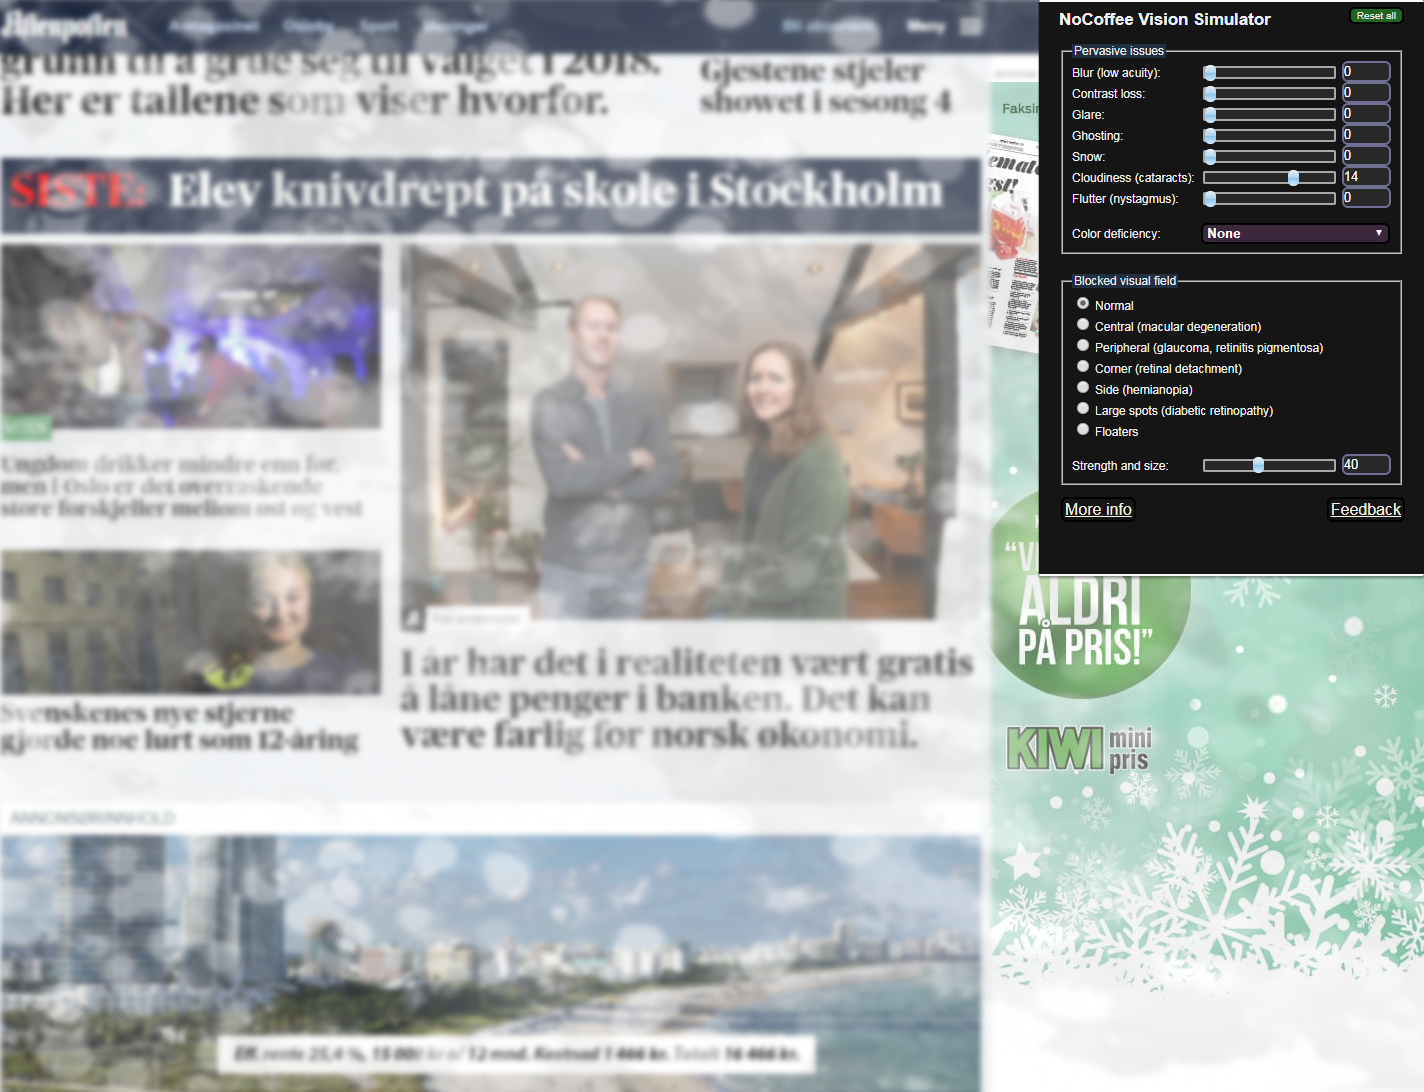
\includegraphics[width=\linewidth]{img/nocoffee.PNG}
          \caption{\textit{The Chrome extension "NoCoffee" simulates different vision impairments by adding a filter on the screen.}}\label{fig:nocoffee_browser_extension_theory_1}
        \endminipage\hfill
    \end{figure}
    \item Simulation using wearable
    
    Vision impairment simulators such as Cambridge simulation glasses and Blue Label Goggles, gloves for simulating dexterity impairments and earplugs for simulating hearing impairments.

    % take own images of cambridge glasses and insert here    
    % \begin{figure}[H]
    %     \minipage{0.8\textwidth}
    %       \includegraphics[width=\linewidth]{src/img/cambridge_simulator.jpg}
    %       \caption{The interface of the Cambridge Capability Loss simulator. Diabetic Retinopathy is selected.}\label{fig:cambridge_simulator_interface}
    %     \endminipage\hfill
    % \end{figure}
    \item Expert testing
    
    Heuristic evaluation where experts evaluates a UI against a set of accepted accessibility heuristics/principles. The authors also includes persona walk-through and cognitive walk-through.
    
    \item Testing with users
    
    Testing a UI on real people. The authors claims that it can be time consuming to recruit subjects and that the most critical accessibility flaws needs to be solved before involving users. 
\end{itemize}

In this thesis I will focus on experience based software simulation, a mixture of \textcite{bai_evaluation_2016}'s "automatic" and "simulation using wearable". More on this in section \ref{discevalsect}.

\section{Universal Design in ICT projects}
\textcite{fuglerud_link_2013} states that although guidelines such as WCAG 2.0 is a precondition to achieve an accessible solution, it might not always be enough. A solution might be technically or theoretically within the requirements of universal design, but still be difficult to use. Some research suggests that WCAG 2.0 only covers around half  of the issues encountered by visually impaired users \parencite{fuglerud_link_2013}.

In the past decade, there has been an increased focus on integrating usability in the software development process \parencite{bai2017cost}. Usability is the focus of the quality and the ease of use of a product. Many companies see the value in making sure their products are user friendly,  and spends resources on usability testing in ICT projects, even though usability testing can take around 8-13\% of the total budget of the project \parencite{bai2017cost}. The incentive for doing this can be that solutions which are difficult to use or are hard to understand makes the user find better alternatives. 

\textcite{bai2017cost} argues that the same focus should be on accessibility testing, even though the cost for user testing for accessibility can be higher then testing for usability, because of the recruitment and accommodation of people with various forms of disabilities can be harder.  

\textcite{fuglerud_link_2013} also argues that projects who has a goal of meeting universal design guidelines should follow a user-centered design methodology. They categorise key elements for having an inclusive design process:
\begin{itemize}
\item "Include multidisciplinary skills and perspectives, 
\item adapt and apply accessibility guidelines and standards,   
\item iterative development, 
\item focus  on  users  with  diverse  accessibility  needs  and  their  usage  contexts  early  and  
\item throughout the development process, 
\item evaluate designs with elderly and people with disabilities, and 
\item focus on the whole user experience."
\end{itemize}


In a utopian project, both usability testing and accessibility testing using real users are done, making sure the solution is user-friendly and accessible for as many people as possible. In reality, time and budget constraints can make it hard to integrate accessibility user testing in projects \parencite{bai_evaluation_2016}. 

\section{Simulations}
\textcite{GoodmanDeane:2007it} claims that although inclusive design provides great benefits for every user of the end product, this can be difficult to achieve in practise. It can be hard to understand the diversity of needs users with different disabilities have, and to estimate the impact different design decisions have on these user groups. Using simulations, some of these obstacles may be overcome.

\subsection{Software simulations}
Software simulation of impairments can demonstrate the effects some impairments have while using screen-based devices. According to \textcite{GoodmanDeane:2007it} software simulators can "help the designers to understand and empathise with the difficulties that less able users might experience when using their products and interfaces". 

\subsection{Critique on using simulators}
\textcite{GoodmanDeane:2007it} is clear on the fact that simulation does not convey the long-term limitations of living with a visual or hearing impairment, such as frustration or coping strategies, but it can give a short insight into the functional experience of having such an impairment. According to \textcite[3]{bai_evaluation_2016}, "the lack of awareness about this distinction is why this approach (simulations) has been highly criticized". 

\textcite{GoodmanDeane:2007it} also states that simulations should not be seen as a substitute for real user involvement, but as a way to internalise insight findings and to test a system before real users are involved. 

\subsubsection{Moore's age experiment}
Patricia Moore, which was in her twenties at the time, toured North America between 1979 and 1982 disguised as an old woman. She experienced abuse, discrimination and marginalisation. She was attacked on the street and on a flight an air hostess spilled coffee on her without apologising \parencite{coleman_design_2007}. 


%\subsection{Who should focus on Universal Design?}




% \section{How ICT solutions are developed}
% To figure out why ICT solutions are inaccessible, we have to understand how ICT solutions are 

% Dong et al. identifies two barriers to the adaption of inclusive design practises within industri in the UK. This study was on 


% Begnum states that there are two different approaches to work with universal design, and calles these "cultural stance": the first cultural stance is viewing  

% Begnum has studied how Universal Design is approached by Norwegian experts working on ICT solutions. She suggests that  there seems to be two cultural stances among the experts: technological and user-oriented. The technological stance, she writes, are more oriented towards checklists, automatic tests and expert inspections, while the 

\iffalse

    \section{Programmer-Focused Website Accessibility Evaluations}
    \begin{displayquote}
    "If you want to change some existing code, you have to first change the programmer's mind."
    \end{displayquote}
    
    %This article by \parencite{Law:ProgrammerFocusedWebsiteAccessibilityEvaluations:2005} highlights the need to treat programmers as the end-users of reports made by accessibility specialists, and it is up to them if the recommendations is implemented or not. These recommendations are often overlooked, if they are not "quick fixes". Programmers generally have a tight schedule and have little training in accessibility, so they only see these recommendations as extra work.
    
    %The authors have come up with a process which can overcome the obstacles, called Streamlined Evaluation and Reporting Process for Accessibility (SERPA). It begins by having the accessibility specialist discussing the project goals and needs of the involved members. The reason to do this is to tailor the future recommendations to the team members. The next step is to agree upon the scope of the project. The authors says it is better to focus on, for example, level A of the WCAG-standard. Next step is to generate a programmer-centric report including fixes first, then guidelines. This makes it easier to focus on the website, not the guidelines. Step four includes evaluating the website with screen readers and similar tools. The article is not clear on whether this means to include developers as evaluators.
    
    This article by \textcite{Law:ProgrammerFocusedWebsiteAccessibilityEvaluations:2005} highlights the problem of having accessibility experts suggesting accessibility fixes, normally in long reports, that are not meeting the needs of the programmers that actually implements the fixes. As a result, most suggestions are overlooked. 
        
    The article also suggests a process that considers the whole development process as well as interpersonal characteristics between programmers and managers. The process is programmer-centric and called "Serpa" (Streamlined Evaluation and Reporting Process for Accessibility).
    
    The ultimate goal of any project that is aimed at a wide population (including people with disabilities) is to be usable for the end-user. But the end user of accessibility reports and recommendations are programmers, and therefore these mediums needs to be usable for this target group. 
    
    Programmers usually have these characteristics:
    \begin{itemize}
        \item Little to no usability training
        \item Think web-users thinks like them
        \item Have little time, and have many groups fighting for their attention and time to fix bugs, aesthetic fixes, usability fixes etc.
        \begin{itemize}
            \item A report with thousand small fixes are less likely to be taken into consideration
        \end{itemize}
        \item Management, not accessibility experts, are more respected and taken serious because they are in charge of promotions and raises and should therefore be the ones in charge of which fixes should be implemented.
    \end{itemize}
    
    The article suggests that it is easier to change the programmers way of thinking then it is to get them to implement accessibility fixes. It is also highlighted that incorporating fixes from the beginning rather than retrofitting (fixing accessibility issues that already are in production), are much better, but that this article is concerned with retrofitting, as this is what most accessibility experts are involved with today.
    
    The last part of the article suggest a programmer-focused process called SERPA. The main parts of this process is:
    \begin{itemize}
        \item Discuss the needs and project goals with all team members.
        \item Agree on the scope and resources.
        \item Fixes could be based on some of the parts of the WCAG Guidelines but not all.
        \item Prepare a programmer-centric report template.
        \item Suggested fixes should be clear first, not accessibility guidelines.
        \item Separate fixes based on content and fixes based on the code / implementation.
        \item Alternative tags are a responsibility of content-creators, not programmers.
        \item Presenting content-related fixes to programmers may be counter-productive.  
    \end{itemize}
    
    \subsection{Outtakes} 
    This article can give me some insight into how some developers think, and how to make accessibility issues relevant to them. It can help me to make design decisions, and to formulate suitable questions for interviews.

\fi
\section{Existing solutions}
\subsection{Cambridge University Capability loss simulation toolkit}
To provide a way to empathise with people having different disabilities, Cambridge University has developed a set of simulation tools they call "Capability loss simulation". The simulation toolset consists of glasses and software that simulates vision impairments and gloves which simulates fine motor-impairments (such as arthritis).

\subsubsection{Impairment simulation software} \label{Impairment simulation software}
The impairment simulation software is making it easy to simulate hearing and vision loss. It includes a set of example pictures and audio files. The software simulates four levels of hearing loss, and several visual impairments and conditions. It is also possible to import pictures into the software, but they have to be of a specific file type. 

\begin{figure}[H]
\minipage{1\textwidth}
  \includegraphics[width=\linewidth]{img/cambridge_simulator.jpg}
  \caption{\textit{The interface of the Cambridge Capability Loss simulator. Diabetic Retinopathy is selected.}}\label{fig:cambridge_simulator_interface}
\endminipage\hfill
\end{figure}

\subsubsection{Cambridge simulation glasses}
In the same toolkit as the \nameref{Impairment simulation software} is the "Cambridge simulation glasses" which are meant to simulate vision loss. The glasses blurries the vision of the user, and can provide a way of experiencing how a person with vision loss might experience an interface. The glasses comes in packages of five or 30 pieces, and are meant to be used on top of each other to provide three different levels of vision loss impairment.

\subsection{NoCoffee browser extension}
NoCoffee is a simulator which can be used to simulate different vision impairments. It works by adding a filter on top of the content of the browser interface. The user of the simulator can adjust different settings such as degrees of blurring, ghosting, different types of color blindness etc.
\begin{figure}[H]
\minipage{1\textwidth}
  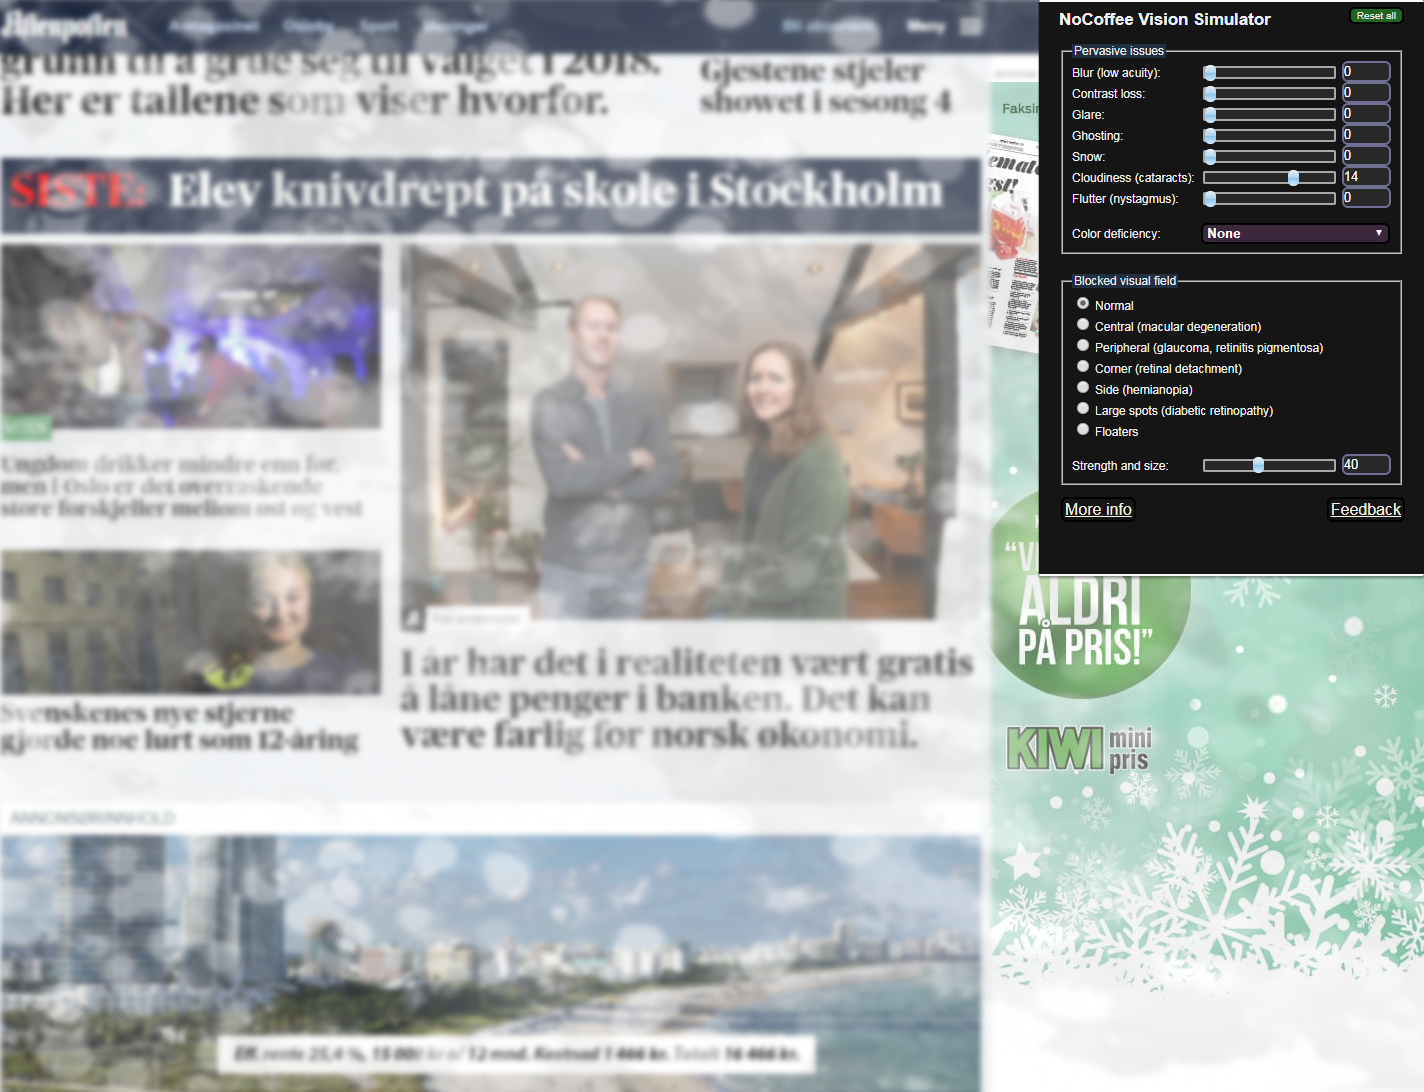
\includegraphics[width=\linewidth]{img/nocoffee.PNG}
  \caption{\textit{The Chrome extension "NoCoffee" simulates different vision impairments by adding a filter on the screen.}}\label{fig:nocoffee_browser_extension_theory_2}
\endminipage\hfill
\end{figure}

The maker of the simulator has posted some thoughts on limitations of the simulator \parencite{_nocoffee_2013}:
\begin{itemize}
    \item The simulations are not medically/scientifically accurate.
    \item The simulations of partial visual fields cannot follow your eyes.
    \item Settings are not linked to statistics and can be hard to relate to
    \item The simulator only works in Chrome
\end{itemize}

\subsection{Funkify browser extension}
This simulator is personas based, meaning that each setting is based on an imaginative person who has a certain impairment: "Blurry Blanca" has blurry vision, "Dyslexia Dani" has dyslexia and "Color Carl" is color blind. The simulator has eight different profiles, all portraying different kinds of impairments.
\begin{figure}[H]
\minipage{1\textwidth}
  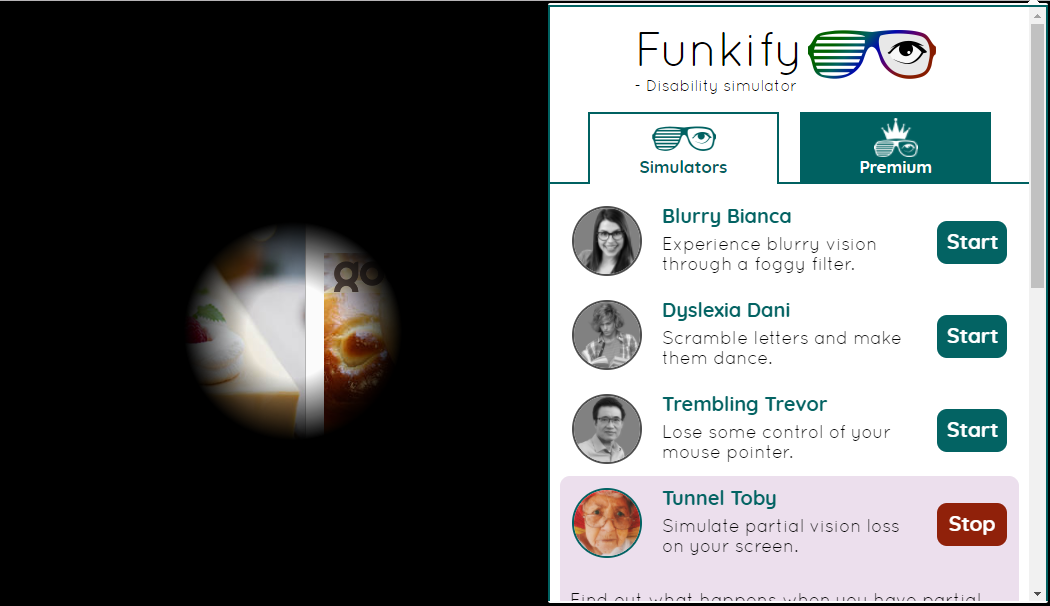
\includegraphics[width=\linewidth]{img/funkify.png}
  \caption{\textit{The Chrome extension "Funkify" simulates different vision impairments and showcases them using personas. Selected are "Tunnel Toby" simulating tunnel vision. The tunnel vision follows the mouse.}}\label{fig:funkify_tunnel}
\endminipage\hfill
\end{figure}
The simulator is created by usability and accessibility experts in Sweden and financed by The Swedish Post and Telecom Authority \parencite{funkify.org_funkify_????}\\

\noindent
The simulator provides statistics on how many people are effected on most of the disability personas.
\begin{figure}[H]
\minipage{1\textwidth}
  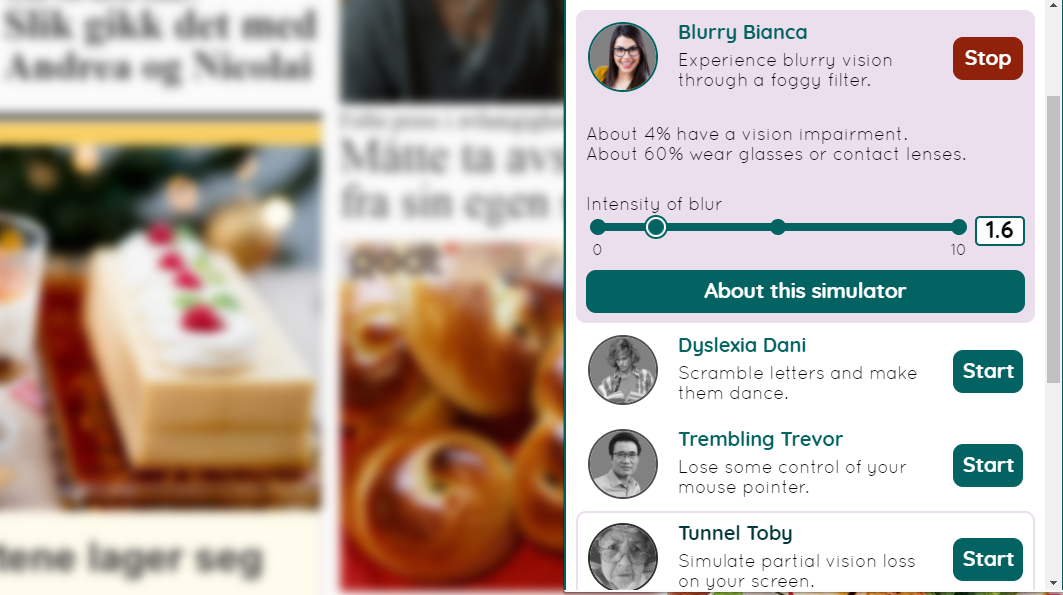
\includegraphics[width=\linewidth]{img/funkify_stats.png}
  \caption{\textit{Statistics are provided to quantify how many people are affected by each impairment.}}\label{fig:funkify_statistics}
\endminipage\hfill
\end{figure}

In figure \ref{fig:funkify_statistics} the persona "Blurry Bianca" is selected. The user of the simulator is provided information that around 4\% of the population has a vision impairment and that 60\% uses glasses or contact lenses. 

%\part{The project}
\chapter{Methods}



This thesis belongs in the critical research paradigm. According to \textcite{myers_set_2011} critical research in information systems is "...concerned with social issues such as freedom, power, social control". 

As the theme of my research question is to question why so few ICT solutions in Norway are meeting the requirements for Universal Design, and that the goal of Universal Design of ICT is to provide equal access to ICT services for most individuals of a society, the critical paradigm is a good fit for this project. 

I am also interested in the target users view on atypical users and universal design, as well as to see if simulations can be a way of motivating the target users to create universal designed ICT solutions. // passer kanskje ikke her

Critical research aims to help realise human potential by "...eliminating causes of unwarranted alienation and domination" \textcite{myers_set_2011}. In this context, elimination of causes of unwarranted alienation and domination would be to figure out how to software simulation can help the target users in making ICT solutions which follows Universal Design guidelines. 

%"...the design of products and environments to be usable by all people, to the greatest extent possible, without the need for adaptation or specialised design" \parencite{miljoverndepartementet_t-1468_2007} this research is indeed critical.

%Placing the research in the interpretive area of research means that I am interested in how 



%I'm placing my research in the interpretative area of research, as I want to understand, not measure people.

%intervjuer
%eksperter
%
%\chapter{Methods}

\section{Focus Group}
Focus groups are simply a gathering of people who can discuss experiences and thoughts about specific topics with a researcher and each other \textcite[90]{CrangMike2007De}. These groups can sometimes have contradictory views, which can be a good thing. Contradictory and competing views can enable "spaces of resistance" where collective knowledge generation can happen \parencite[90]{CrangMike2007De}. 

To enable more participants to argue or discuss and reflect over a given topic can be valuable, both for the participants and for the researcher. The probability for whether these spaces of resistance can occur, relies on the group dynamic. It can be an advantage to recruit people who know each other if the goal is to study this group in particular. However, according to \textcite{CrangMike2007De}, recruiting strangers can facilitate the discussion to be more like the one they might have with strangers and encourage shy participants to be engaged in the conversation if less shy members "break the ice".

Whether the group is homogeneous or heterogeneous regarding gender can also impact the group dynamic and discussion in the focus group. Men have a tendency to "speak to the crowd" while women tend to break into one-on-one conversations which are lost to the group as a whole \parencite[92]{CrangMike2007De}.

\section{Interviews}
Interviews are usually categorised as unstructured, structured and semi-structured (Fontana and Frey 1994 in \cite{rogers_interaction_2011}). The choice of interview type depends on the research question and the goal of the interview.

\subsection{Expert interviews}
According to \citeauthor{meuser2009expert}, expert interviews can be an effective method of inquiry because an expert can be seen as "surrogates for a wider circle of players" \parencite[2]{meuser2009expert}. Especially in the exploratory phase of a project, expert interviews can be an efficient point of entry into the research area and can provide clues on where to go for further inquiry.  

An expert is someone who has has expert knowledge of a subject and is distinguished from someone with "everyday knowledge and common-sense knowledge" \parencite[18]{meuser2009expert}. Who is identified as an expert is up to the researcher's judgement (ibid). 

Experts can inherit experiences, insider knowledge and domain knowledge about a subject. Experts can also be motivated to provide the researcher with knowledge to "make a difference" about the area of research or be motivated out of professional curiosity \parencite{meuser2009expert}.

\section{Casting the net}
%\section{Background activities}
Before conducting any empirical activities, I have investigated the topic through some background activities. I have observed a focus group held by students at my faculty, I went to an experience conference where the topic was Universal Design and I went to a meetup event held by an interest group called “Universal Design and digital inclusion”. Details on these activities are found in chapter xx.xx.

\subsection{Focus group with inexperienced developers}
The aim of the focus group was to look at the views and knowledge inexperienced developers had on Universal Design. The reason I went to this focus group was to get a better understanding of the views developers has on the subject of Universal Design and to get ideas on where I might steer the thesis.

Many of the participants had heard of Universal Design, but few knew exactly what it means or how to implement it. The developers did as they were told by their project leaders, and if they were requested to implement an accessibility fix, they did that. Some participants requested a better focus on Universal Design in higher education, as it would make their jobs easier if they had had more about the topic during their education.

\subsection{Experience conference}
I went to this conference to get a better understanding of Universal Design and how other fields (not related ICT) talk about this topic. I heard talks by architects, project managers and others who all had the same goal: to create a more inclusive society. 

Experiences I took from this conference:
\begin{itemize}
\item In all fields that can influence the experience people with disabilities might have with the world, there is a need to focus on Universal Design, especially in the education system.
\item On this conference they focused more on the inclusion of all members of society, but not on minimal requirements such as ramps and accessibility tools. 
\item The dogma on this conference seemed to be that facilitation for everyone, not just people with disabilities can benefit the society as a whole. In the opening statement, Helge Eide said: “Universal Design makes it possible for most people to participate in society as long as possible”. 
\item It was also mentioned that a visionary view on Universal Design can prohibit the evolution of the concept, and that we should focus on concrete examples. Universal Design must move from something you talk about in “party speeches” to something that happens in practise.
\item All Norwegian municipalities are obligated to have a council for people with impairments consisting of users with disabilities, politicians and representatives from the municipality. The council usually function as evaluators of solutions, but for this to work properly, this council should be included at the start of projects. 
\end{itemize}

The experience conference left me with the impression that there is a struggle to make the world accessible for all, but that this struggle will diminish if there is more focus on the topic in education programs for people who has a direct influence in artefacts and environments. It also left me with the impression that there often is a focus on minimal requirements in building projects so as not to break the law, but that many universal design enthusiasts requests a thorough understanding and inclusion of accessibility requirements early in the planning phase of the project.

These reflections can also be made in regards to ICT-solutions which often focus on Universal Design late in projects, if it is a focus at all. 

\subsection{Meetup with "Universal Design and digital inclusion"}
To get a glimpse into how the culture is amongst accessibility enthusiast, I went to a meetup organised by the Facebook group “Universal Design - best practises” which I was invited to by a informant I interviewed earlier in the project. 



\section{Litterature review}
I have reviewed litterature from several sources. Mainly, I have found articles on ACM and Sage JournalSage Journal




%[TODO: implement theory into the description of the focus group]




\subsubsection{Interview with Universal Design Enthusiast}
% \subsection{Location}
An expert interview was held at a café November 16. 2017 in Oslo city centre. The expert interview was held in relation to the course "INF5261 - Development of mobile information systems" by me and my two group members project in that course. The project had the same theme as this thesis, and the information uncovered in this interview is therefore relevant to this thesis as well. We were three researchers and one participant present during the interview.

The interview was based on an interview guide we had prepared in advance. The interview guide was designed with inspiration from \textcite{tone_nordbo_introduksjon_2017}.

\subsection{Ethics}
A consent form was used to inherit the participant's anonymity and to inform him about the purpose of the interview and the research project. The consent consisted of information about the purpose of the interview, what happens to the information uncovered in the interview, and our contact information - in case he had any questions at a later time. It also informed the participant that he could at any time withdraw from the study without any reason or repercussions. The subject was sent the consent form the day before the interview, so he could read the document in peace and not feel rushed to sign something he was not fully aware of.

\subsection{Participant}
Our expert currently worked as a consultant at a renowned Norwegian firm as a senior front-end developer consultant and manager. He has previous experience in leading a Universal Design disciplinary group at his firm, and considers himself a Universal Design enthusiast. The expert was familiar with MediaLT from collaborating with them on earlier projects.

\subsection{Recording}
The interview was not recorded by audio or video equipment. One of the researchers acted as an observer and note-taker and did not participate in the interview. 

\subsection{Questions}
This is a brief overview of the themes discussed in the first expert interview. For more details, see xx Interview Guide or %\ref{ap-2-expert-interview-1}. 
The interview guide consisted of the following themes:
\begin{itemize}
    \item Introduction and background
    
    Presenting the informed consent form. Present the researchers, time frame, note taking and basic information about the participant.
    
    \item Education
    Asking how the expert got into UU and when they were made conscious about UU.
    
    \item Practising
    
    How the developers in the experts company learns about UU.
    \begin{itemize}
        \item How do you work with Universal Design in your company?
        \begin{itemize}
            \item Insight
            \item Prototyping
            \item Evaluation
        \end{itemize}
    \end{itemize}
    \item Whip or carrot
    
    Asking if laws and repercussions are the best way to make more people focus on UU.
    
    \item Possible solutions
    
    Discussing possible solutions.
\end{itemize}

\subsection{Focus Group with developers}
I participated at a focus group as an observer 03. October 2017. The goal of the focus group was to explore if and how developers relate to Universal Design. This focus group was held by a group doing a project with MediaLT in the course "INF5261 - Development of mobile information systems and services" at the University of Oslo, which I also took at the time.

This focus group was not held by me, I had no impact in the recruitment of the participants, discussion, questions asked or themes brought up. I was mostly an observer. However, I was asked if I knew of any female front end developers that they could recruit to the focus group.

\subsection{Participants and recruiting}
There were 7 participants in the workshop. All of the participants were males between 20 and 27. Most of the participants was working as front-end developers, one were studying programming, and one was looking for a job as a back-end developer. One participant was working as Staffing Manager, and had to consider Universal Design when he accepted projects. All the participants had or was undergoing a bachelors degree in information technology.

The participants were contacts of the students who held the focus group. Most were previous classmates of two of the students who held the focus group.

All the participants were male, but this was not a conscious decision by the focus group-holders, they wanted to recruit more females to balance the discussion.

\subsection{Moderation}
In the focus group, one of the students acted as a moderator. She introduced the theme of the focus group and guided the discussion.

\subsection{Group dynamics}
In the focus group, some people were more audible than others. The moderator did a good job in letting everyone participate in the discussion, and was also actively including all the members by asking them what they thought about the themes discussed.



\subsection{Interview with researcher}
The researcher I interviewed has been working as a backend developer before he decided to become a researcher. His interest field is, amongst other, Universal Design.

\subsection{Interview with developer}
I contacted a person 
\chapter{Case}
\section{MediaLT}
MediaLT is a Norwegian company concerned with making the web accessible for most people, including people with different kinds of disabilities. They provide training in (among other things) Universal Design and they analyse and comes with suggestions on websites regarding Universal Design principles and implementation.

\section{Stable Test Sites}
This master thesis is related to MediaLT's project "Stable test sites" which came together after Difi in 2016 wanted an overview of how reliable automated testing tools are for measuring WCAG 2.0 success criterion. They found out that the only way to measure this was to find inaccessible websites and see if the automated test tools would react on the errors. They soon found out that this was a tedious job, and that it would be much smarter to make their own inaccessible websites that could measure the WCAG 2.0 success criterion.

This thesis is focused on making Universal Design principles relevant for developers, make it easier to learn about Universal Design principles and to ultimately on their own be able to identify accessibility issues that automatic testing tools fails to identify.

\section{Users}
\textit{Users} in this thesis are front-end programmers, interaction designers or graphic designers, who to some extent has an influence on how an ICT solution aimed at a general population can be designed or implemented. The most relevant users has an ongoing project where they need to cater for universal design in their solution, but as I am also interested in the target users views on disabilities and universal design, all professional designers or front-end developers are target users. 



%\part{Results and discussion}
\chapter{Findings}

\section{How do developers learn about accessibility?}

\subsection{Relatable examples to gain interest}
Stian uses examples that everyone, whether you have a disability or not, can relate to when he teaches accessibility. These examples are to motivate accessibility and universal design is important. Examples he uses:
\begin{itemize}
    \item Sun glare on computer screens to demonstrate the issue of having enough contrast between elements.
    \item Wanting to watch a video without a headset to demonstrate the need for subtitles.
\end{itemize}

Stian has also used parkinsons gloves that has a spinning motor simulating parkinsons disease and Cambridge Glasses on a stand at internal seminars. The people who came to the stand were asked to use a smartphone with the Parkinson gloves and to read on a poster with text with varying contrast levels between the text and the background. Stian notes:

\begin{displayquote}
    With the glasses you can't see anything under the requirement level.
\end{displayquote}

Stian also uses examples because going straight into the requirements and laws would be detrimental.

\begin{displayquote}
    It is quickly more interesting for developers to follow examples rather than rules and requirements. It is ironically very difficult to learn about all the Universal Design requirements. It is hard to relate to them. I don’t think WCAG 2.0 is easy, but now I have used it so much, so I am used to it. When I started with it, it was hairy.
\end{displayquote}

Stian notes that actually experiencing what thinking about accessibility  (or the lack of it) can do is much more effective than reading about requirements.

\begin{displayquote}
    To see someone struggling with the amazing thing you think you have built helps and creates engagement - builds empathy. Instead of reading about it, experience it. It has a much bigger effect.
\end{displayquote}

\subsection{Prestigious}
Stian says that when he got interested in accessibility it was prestigious to make semantic and validated HTML code. Writing semantic and validated HTML code often solves many accessibility related problems. \textcite{sandnes} says: "Computer students are often fascinated by achieving near impossible things, being it novel and effective algorithms, making hardware do things it was not meant to, etc". Sandnes uses this as an approach to develop a positive attitude amongst computer science students toward universal design.

%The general impression I got from watching developers use the empathy tools, was that they had fun. They were joking and laughing and seemed to enjoy doing it. 

\section{How do developers learn accessibility?}

\subsection{Enthusiast driven}
Stian says that some developers learns about universal design and accessibility in ICT projects, but that it relies heavily on having an enthusiast on the team that knows about it and is willing to share his / her knowledge to the rest of the team. Lars has also seen the importance of enthusiasts in ICT projects 

\begin{displayquote}
    (...) we have seen that if you have one enthusiast that can make sure you always have some focus on it if you forget about it in a project or in a company.
\end{displayquote}

Lars mentioned an enthusiast who had struggled with convincing his management to focus on universal design from the start rather than retrofitting in the late stages of the projects. The enthusiast had gone so far as to organise three projects which were quite similar and he instructed one of them to focus on universal design from the start, and the others to not focus on it. The project which focused on it from the start used 15\% less money then the project that had to retrofit implementation of universal design. The person who initiated this experiment did it to get hard numbers as arguments on why they should focus more on Universal Design.

\subsection{Random entry}
Lars says that you have no relation to universal design or accessibility if you have not gotten a task that governs it. He says the way into the field seems random. *


\section{The use of empathy tools}
Using empathy tools conveyed frustration, relief and surprise. Karl was using Keyboard Kim to order a ticket on SAS, when he got cought in a different ticket then he was going for.

\begin{displayquote}
    Oh, how does this work? What I did was that I entered the meny and I noticed that the radio buttons that I was going to use was not that easy to select from.
    
    There. Oh, I have to use the arrow keys, then. Oheh, help. I was caught in a flexible ticket. Because when I'm activating this choice, my pointer disappears. What I think I do now is that I go from 08:20 in the morning. I can't scroll by the way. Like that. Then I go back 19:35.
\end{displayquote}

Karl noticed many errors in the interface, and was not shy to express his frustration. When he had tried to buy a youth ticket for a while without succeeding, I said that we could move on.

\begin{displayquote}
    Yes, but I have to do those choices. Oh my god. It traps me all the time. It is just awful. There.
    
    Yes. Then... Ah, come on now. Then I go to order.
\end{displayquote}

It was clear that it was important for him to succeed at his task.


\chapter{Discussion}
Sven cannot expect the Norwegians he meets to speak Swedish to him, and Norwegians can't expect Sven to understand all the dialect words they might normally use in conversations with other Norwegians. This mutual understanding comes from interacting with each other.

At the same time, developers can't expect every user to have the same functional capabilities as themselves. Using empathy tools they can get a sense of which barriers the solution might have. If the alternative is that the developer has no contact with real users, empathy tools is definitely a good alternative. The best alternative is for the developer to see how people with different capabilities other then themselves are using the ICT solution.

\section{\textit{How to make accessibility issues more apparent for developers?}}
%How can we make the use of
\section{Relatable examples}
Stian's use of relatable examples in his teaching can give the developers some perspective before they are exposed to the legal requirements. Instead of focusing on requirements and how to make ICT solutions that are legal and functional accessible, he uses examples where everyone could benefit of more universal designed solutions.




\section{\textit{Can empathy tools motivate developers to consider the needs of people with different capabilities?}}




\section{\textit{How does the use of empathy tools impact developers?}}

%\section{\textit{Which kinds of empathy tools are best suited for developers working on ICT
%solutions?}}

\subsection{\textit{Which kinds of empathy tools are best suited for developers working on ICT
solutions?}}
For simulators to be a tool for developers, it needs to be accurate and integrated in the current environments of the developers.

\subsection{Cost effective}
Cutting costs and saving time is an important aspect of ICT projects.

\begin{displayquote}
    People are always concerned with cutting costs. There are no-one that, unless they need to or make money of it, do something. That's how the reality is. We want to do the best job, in a pragmatic way. But the customer has their budgets to relate to that they might not be in charge of themselves.
\end{displayquote}
With this in mind, for a simulator to be useful for developers it would need to be calibrated with statistics so that developers are sure to include the widest range of possible end-users, and that the solution is within the legal requirements. 

\begin{displayquote}
    I know there is a list, and that not all the requirements need to be fullfilled. So it would be cool if you could turn on WCAG requirements based on where you are, Norway, America and so on. 
    
    I think that is very relevant, especially for professional use. This [Funkify and Cambridge glasses] is cool as a thing, but if you are selling it to professional use, you have to be able to configure this after the teams needs.
\end{displayquote}

\backmatter{}
\printbibliography
\end{document}